\documentclass[10pt]{article}

\usepackage{hyperref}
\usepackage{amsthm}
\usepackage{amsmath}
\usepackage{amsfonts}
\usepackage{graphicx}
\graphicspath{ {./images/} }

\theoremstyle{definition}
\newtheorem*{problem}{Problem}

\setlength\parindent{0pt}

\newcommand{\R}{\mathbb{R}}
\newcommand{\Z}{\mathbb{Z}}
\newcommand{\snorm}[1]{\lVert#1\rVert}
\newcommand{\abs}[1]{\left|#1\right|}
\newcommand{\sgn}{\mathop{sgn}}
\newcommand{\diag}{\mathop{diag}}
\newcommand{\inp}[2]{\left\langle#1, #2 \right\rangle}
\newcommand{\vspan}{\mathop{span}}
\newcommand{\var}{\mathop{var}}
\newcommand{\E}{\mathbb{E}}
\newcommand{\Null}{\mathop{Null}}
\newcommand{\Row}{\mathop{Row}}
\newcommand{\dd}[2]{\frac{d#1}{d#2}}
\newcommand{\rank}{\mathop{rank}}



\title{Alg Top: Informal Reading Group\\ Meeting 1.}
\date{Updated: \today}
\author{\href{tsawada7@gatech.edu}{Tom Sawada}}


\begin{document}

\maketitle


\begin{problem}[3.C.4]
\textbf{$H$-spaces.}\ Let $(X,e,\mu)$ be an $H$-space. We claim that the universal cover $p: \tilde{X}\to X$ has an $H$-space structure. Let $\tilde{e}$ be any lift of $e$. Since $\tilde{X}\times \tilde{X}$ is simply connected, we can lift the map 

\begin{equation}
	\mu\circ (p\times p): \tilde{X} \times \tilde{X}\to \tilde{X}\times \tilde{X}
\end{equation}


so that the diagram commutes: 

\begin{figure}[h]
% \caption{}
\centering
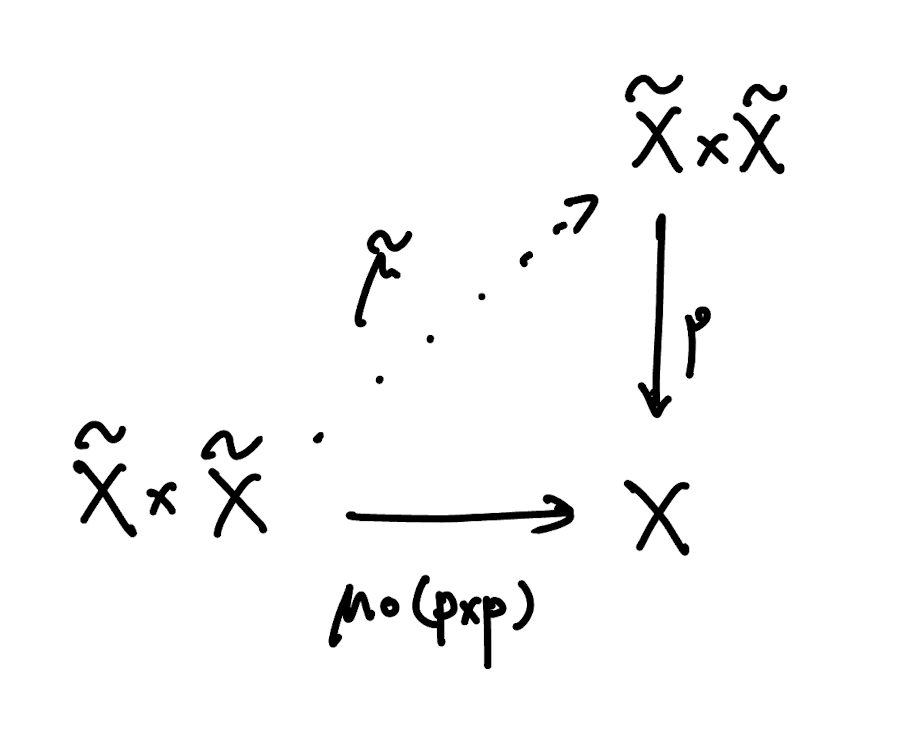
\includegraphics[width=0.2\textwidth]{image/3c4_mutilde_def.png}
\end{figure}


To show that $\tilde{\mu}$ satisfies the axioms of an $H$-space, apply the homotopy lifting property to the map 


\begin{equation}
	F: \tilde{X} \to X
\end{equation}

\begin{equation}
	\tilde{x}\mapsto \tilde{\mu}(\tilde{e},p(\tilde{x}))
\end{equation}

\begin{figure}[h]

\centering
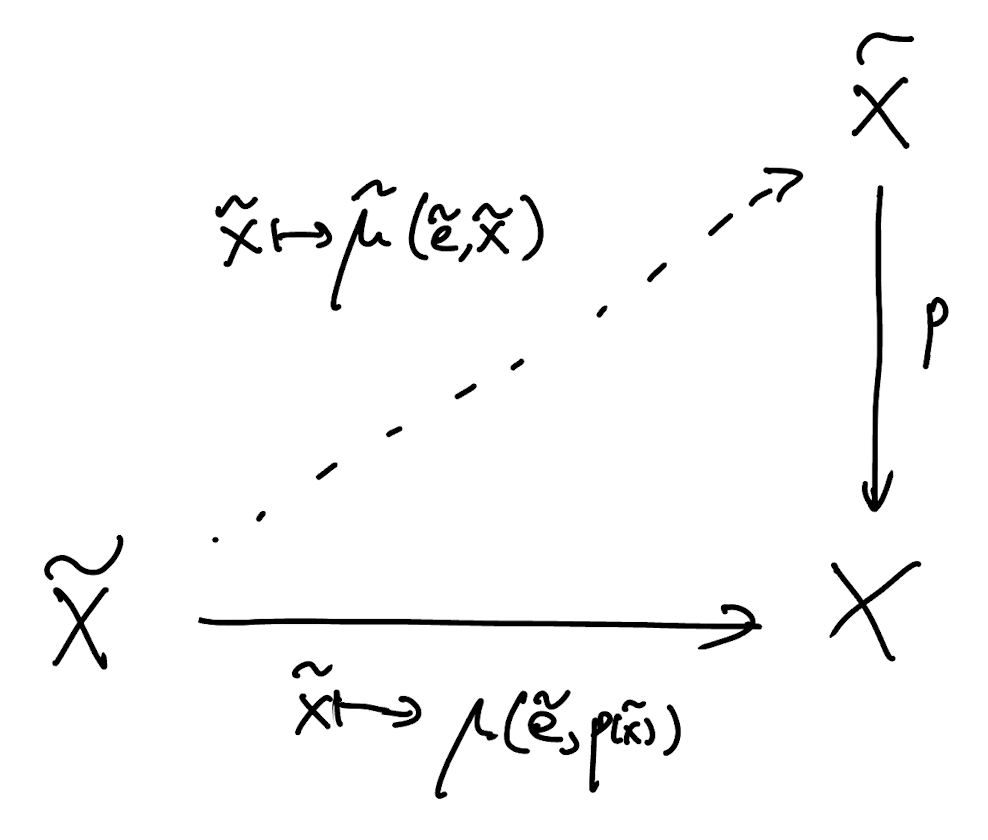
\includegraphics[width=0.2\textwidth]{image/3c4_homotopy_lift.png}
\end{figure}

Since the map $y \mapsto \mu(e,y)$ is homotopic to the identity, the map $\tilde{x} \mapsto \tilde{\mu}(\tilde{e},\tilde{x})$ is also homotopic to the identity.\qed\\



% We claim that $\tilde{\mu}$ satisfies the axioms of an $H$-space. Let 

% \begin{equation}
% 	H: X\times [0,1] \to X
% \end{equation}

% be a homotopy between $\mu(e,x)$ and the identity map $I_X$ on the space $X$, so that $H_0 = \mu(e,x)$ and $H_1 = I_X$. Then consider the composition 


% \begin{equation}
% 	H\circ (p\times I_{[0,1]}): \tilde{X}\times [0,1] \to X
% \end{equation}

% \begin{equation}
% 	(\tilde{x},t) \mapsto H(p(\tilde{x}),t)
% \end{equation}

% Since $\tilde{X}\times [0,1]$ is simply connected, by the lifting criteria, the above map lifts to $\tilde{X}$: 

% \begin{figure}[h]
% % \caption{}
% \centering
% 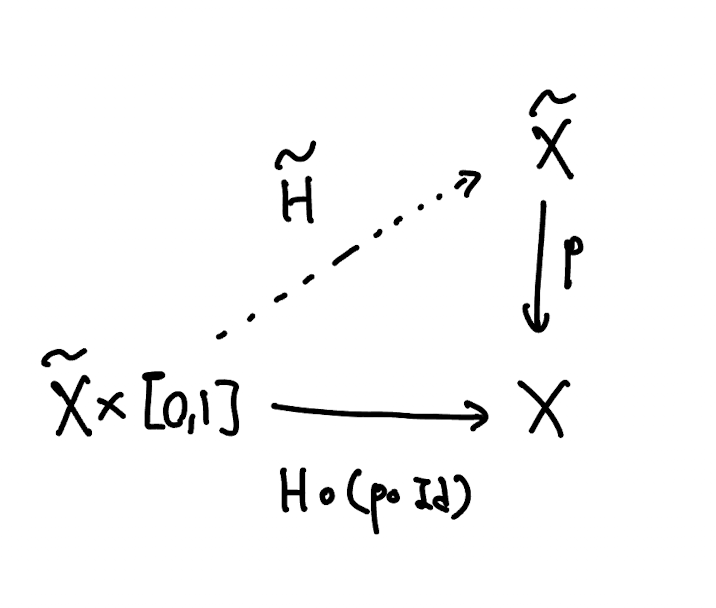
\includegraphics[width=0.4\textwidth]{image/3c4_homotopy_def.png}
% \end{figure}
% \vspace{2em}

% Since the diagram commutes, $\tilde{H}(\tilde{x},0) = \tilde{\mu}(\tilde{e}, \tilde{x})$





	
\end{problem}


















\end{document}